\documentclass{article}
\usepackage[T1]{fontenc}
\usepackage{lmodern}
\usepackage{graphicx}
\usepackage{amsmath,amssymb}
\usepackage[a4paper,margin=2cm]{geometry}
\usepackage[absolute,overlay]{textpos}
\setlength{\TPHorizModule}{1mm}
\setlength{\TPVertModule}{1mm}
\usepackage[indonesian]{babel}
\usepackage{hyperref}
\setlength{\emergencystretch}{2em}
% unit: Halaman 22

\begin{document}

% === Halaman 22 (llm) ===

$S_1$:
\vspace{5mm}
$S_2$:
\vspace{5mm}
$S_3$:
\vspace{5mm}
$S_4$:

\vspace{38.61mm}

% deskripsi: Tabel matriks S1 berisi angka-angka acak dalam grid 4x15
% bbox normalisasi: [0.6600, 0.6600, 1.0000, 1.0000]
\begin{textblock*}{71.40mm}(138.60mm,196.02mm)
\noindent
\includegraphics[width=71.40mm,height=100.98mm]{../../images/llm/page_022_img_01.png}%
\end{textblock*}

% deskripsi: Tabel matriks S2 berisi angka-angka acak dalam grid 4x15
% bbox normalisasi: [0.0400, 0.3000, 0.6400, 0.4400]
\begin{textblock*}{126.00mm}(8.40mm,89.10mm)
\noindent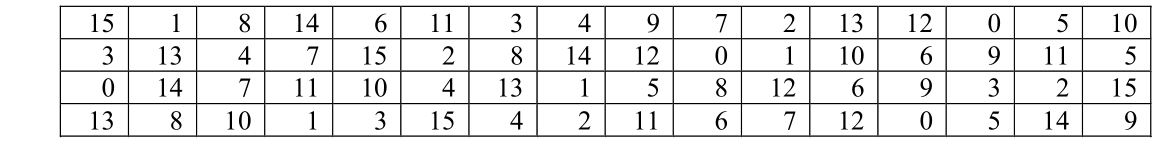
\includegraphics[width=126.00mm,height=41.58mm]{../../images/llm/page_022_img_02.png}%
\end{textblock*}

% deskripsi: Tabel matriks S3 berisi angka-angka acak dalam grid 4x15
% bbox normalisasi: [0.0400, 0.5200, 0.6400, 0.6500]
\begin{textblock*}{126.00mm}(8.40mm,154.44mm)
\noindent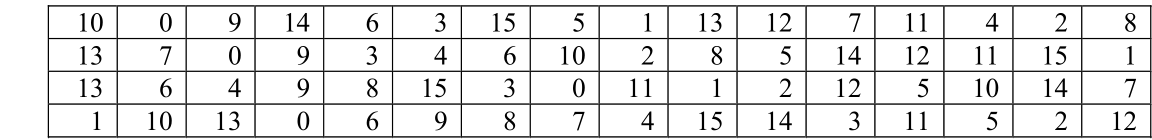
\includegraphics[width=126.00mm,height=38.61mm]{../../images/llm/page_022_img_03.png}%
\end{textblock*}

% deskripsi: Tabel matriks S4 berisi angka-angka acak dalam grid 4x15
% bbox normalisasi: [0.0400, 0.7300, 0.6400, 0.8600]
\begin{textblock*}{126.00mm}(8.40mm,216.81mm)
\noindent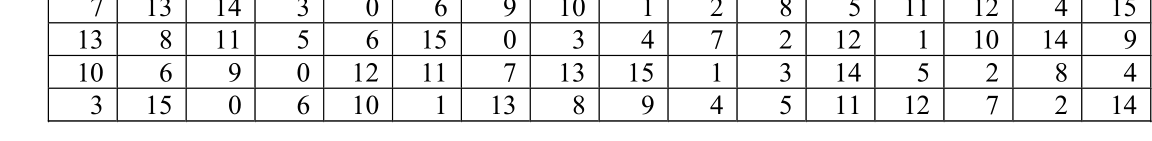
\includegraphics[width=126.00mm,height=38.61mm]{../../images/llm/page_022_img_04.png}%
\end{textblock*}

\end{document}
